
\subsection{Topology of Hidden Markov Models}

Because the Baum-Welch algorithm assumes that the model is correct, it is important to devise a suitable topology before training starts. 
The topology of the model is usually built by using a prior knowledge of the data. 
For handwritten signals, a left-to-right HMM is often used where no back transitions from right to left are allowed. \cite{Suen}

\subsubsection{Hidden Markov Model Topology for the Character Classifier}

A model is created for each character in the training phase, as described in Section~\ref{sec:overview_of_classifiers}.
Because the English alphabet only contains 26 characters, it is not too computationally costly to train a separate model for each character.
The topology is very similar to the topology suggested by Laan et al \cite{Laan}. 
We used special beginning and end states denoted by \textit{b} and \textit{e} respectively.
If the image feature extraction step produces $n$ segments there will be $n + 2$ states in the HMMs.
Special beginning and end states are included because multiple training observation sequences are concatenated to form one observation sequence.
The sequence is then used as input for the Baum-Welch algorithm.
The initialization of the transition and emission matrices are done so the following properties are fulfilled:

\begin{itemize}
 \item The beginning state \textit{b} will always emit the special symbol @ and the end state will always emit the special symbol \$.
 \item The  beginning state \textit{b} always transitions to the first normal state.
 \item The ending state \textit{e} always transitions back to the beginning state \textit{b}.
 \item All other states always transitions forward to a state that has not been visited since the last visit to \textit{b}
\end{itemize}



\subsubsection{Hidden Markov Model Topology for the Word Classifiers}

We have implemented two classifiers for classifying words. 
The first has exactly the same topology as the character classifier and uses one HMM for every character as described in Section~\ref{sec:overview_of_classifiers}. 
If the word has $n$ letters the word there will be $n + 2$ states in the corresponding HMM.

It is natural to implement one HMM for each of the words when the vocabulary is small.
When the vocabulary is larger this approach may have performance problems.
A single model has the additional benefit that it can learn common patterns in words such as ''ing''.

The second word classifier that have been implemented uses a single HMM for the whole vocabulary. 
The HMM used in the second word classifier is called \textit{Word HMM} in the following text.
See \ref{figure:wordtopology}.

\begin{figure}[h!]
\centering
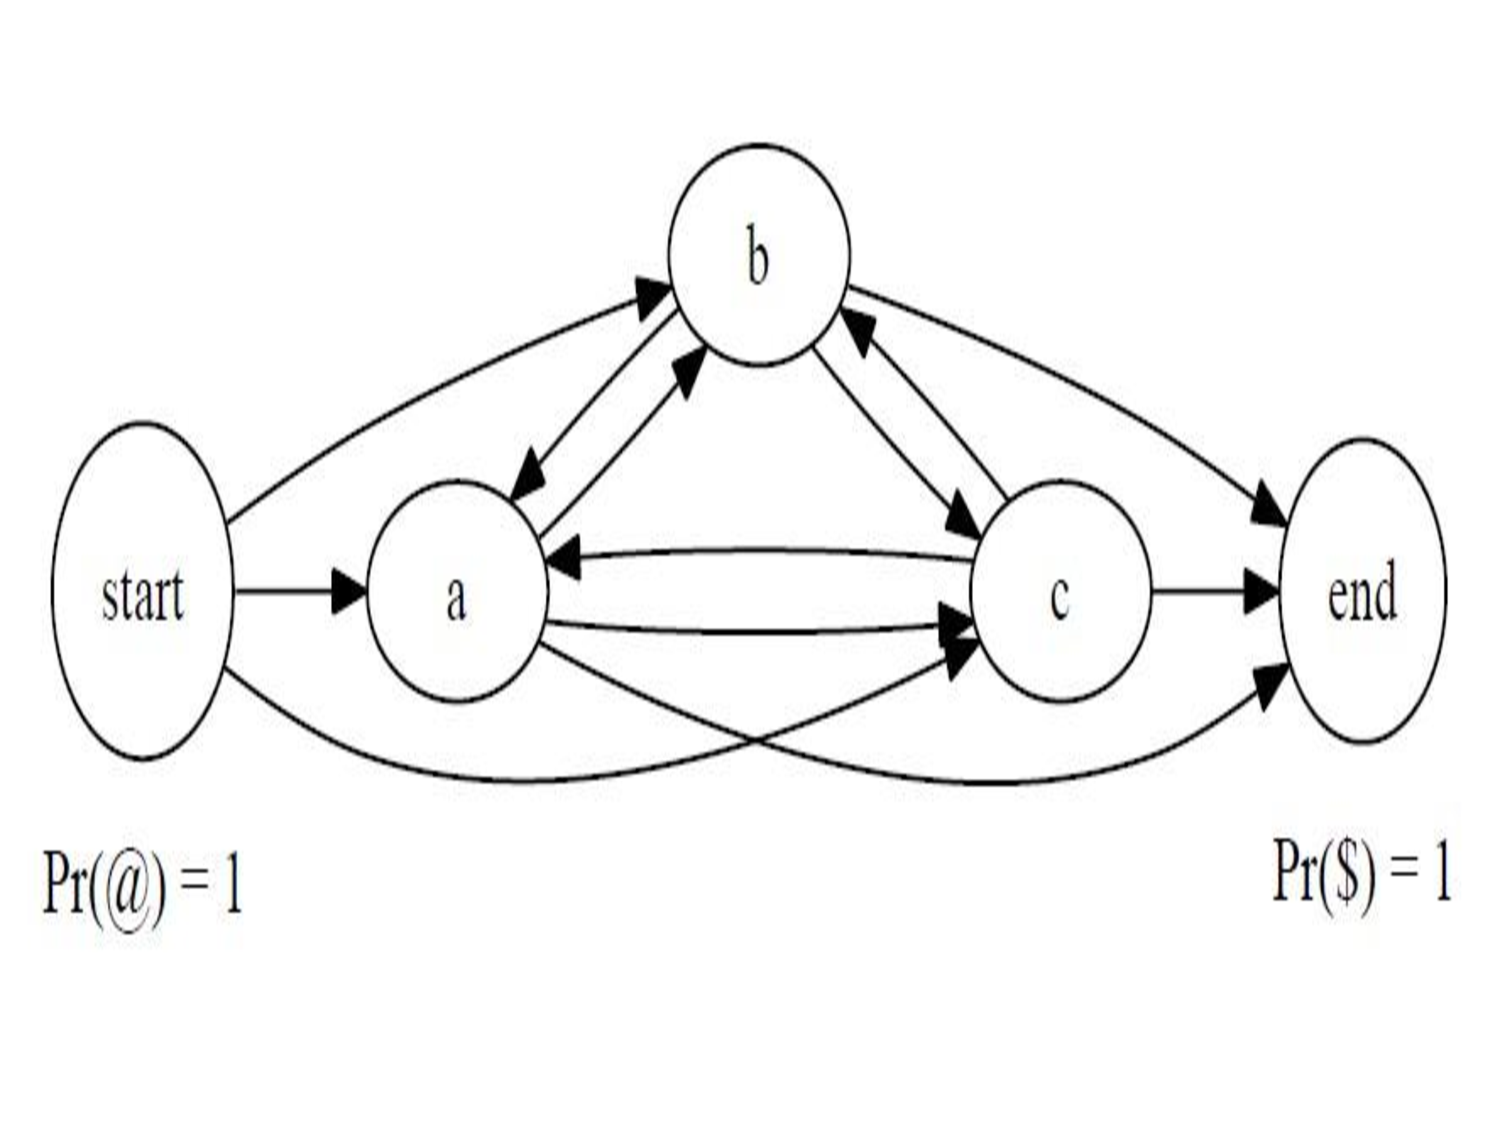
\includegraphics[width=4in,height=2in]{wordtopology}
\caption{Word HMM topology for a three-letter alphabet.}
\label{figure:wordtopology}
\end{figure}

Unlike the HMMs used in the character classifier, \textit{Word HMM} have states that have transitions to all other states.
It has 28 hidden states (26 for the 26 English letters and 2 with special emissions @ and \$). 
The transition matrix is a 28 * 28 matrix, which is estimated from the lexicon analysis.
For example if there are only three words in our vocabulary: DOG, CAT and CAP.
Then the probability of going from A to T is $0.5$, A to P is $0.5$ and A to other letters is set to $0$.

The observations are the letters we have observed from the character classifier.
The observation probability matrix is created from observations done when testing the character classifier.
For example, if we have 10 test example images for A, and 5 of them are classified to be A, 3 to be B and 2 to be C, then $P(observation A)=0.5$, $P(observation B)=0.3$ and $P(observation C)=0.2$.
In that case the row for A in the probability matrix will be assigned to $[0.5, 0.3, 0.2, 0, 0,...,0]$.

\subsection{Initial Parameter Selection}
%4.1. Describe the different initialization algos, advantages and disadvantages. Chongyang

Hidden Markov Models can be efficiently trained by Baum-Welch (BW) algorithm, which is an iterative process for estimating parameters for HMMs. 
As an iterative algorithm, BW starts from an initial model and estimates transition and emission probability parameters by computing expectations via the Forward-Backward algorithm.
The algorithm sums over all paths containing a given event until convergence is reached.

Since the Baum-Welch algorithm is a local iterative method, the resulting HMM and the number of required iterations depend heavily on the initial model. 
There are many ways to generate an initial model, some techniques consider the training data while others do not \cite{Laan}.
Similar to Laan et al. \cite{Laan}, we tried two initialization strategies, count-based and random.
The random initialization strategy assigns the values in the transition and emission matrices to random values.
For the count-based initialization the emission matrix is assigned based on information from the training examples and the transition matrix is assigned so that all states get the same probability of transferring to all states that are reachable.

\subsection{Implementation Issues}

During the implementation of the HMM and related algorithms, we run into some problems. These problems are described in the following sections.

\subsubsection{Floating Point Precision}

When the number of states \textbf{t} grows sufficiently large, the forward variable $\textbf{a}_t(i)$ and backward variable  $\textbf{b}_t(i)$ approaches zero and exceed the precision range of floating point numbers.
One way to solve this problem is by incorporating a scaling procedure.
For each \textbf{t}, we first compute $\textbf{a}_t(i)$ according to the induction equation (20) in  \cite{Rabiner1989}, and then multiply it by a scaling factor  $\textbf{c}_t$, calculated by Equation \ref{eq:rabiner-scaling}, where $N$ is the number of states.
% Maybe we should the explain the equation in more detail.. For example what  N is.

\begin{equation}\label{eq:rabiner-scaling}
\textbf{c}_t = \frac{1}{ \displaystyle\sum_{i=1}^N \textbf{a}_t(i)}
\end{equation}

To avoid the underflow problem in the Viterbi algorithm, which calculates the maximum likelihood state sequence, we add log probabilities instead of multiplying probabilities.
With this change, no scaling is required.

\subsubsection{Zero Probability Transitions}
% We should explain WHY this is a problem.
Another problem that may occur when training HMM parameters when little training data is available, is that the probability matrices may contain zero values for transitions and emissions that actually are possible.
This could lead to bad results if the test set contains a lot of these ''impressible'' transitions.
In the \textit{Word HMM} we initialize all zero probabilities to the value \textbf{ $10^{-10}$}.
For the other HMMs this is left as future work.